%%%%%%%%%%%%%%%%%%%%%%%%%%%%%%%%%%%%%%%%%%%%%%%%%%%%%%%%%%%%%%%%%%%%%%%%%%%%%%%%%%%%%%%%%%%
%%
%% The updated version of this document should be downloaded from
%%      https://github.com/jp-um/university_of_malta_LaTeX_dissertation_template
%%
%% In case of any difficulties please contact Dr JP Ebejer on jean.p.ebejer@um.edu.mt
%%
%%%%%%%%%%%%%%%%%%%%%%%%%%%%%%%%%%%%%%%%%%%%%%%%%%%%%%%%%%%%%%%%%%%%%%%%%%%%%%%%%%%%%%%%%%%

%% Before you embark on this quest you should probably read some of:
%% Deadly sins - http://ctan.mirror.garr.it/mirrors/CTAN/info/l2tabu/english/l2tabuen.pdf
%% Writing a thesis in LaTeX - http://tug.org/pracjourn/2008-1/mori/mori.pdf

\RequirePackage[l2tabu, orthodox]{nag} % tells you of any bad LaTeX usage
                                       % must be first thing in class (with the exception of comments)

%% There is one option you should define; oneside or twoside
%% Use twoside for your viva docs (examiners hate long docs they need to carry around)
%% and oneside for the final thing you submit to the library.  Note that margins will
%% change accordingly

\documentclass[twoside]{mmu}  % custom University of Malta project/dissertation/thesis


%% **************** (Your) Packages (Start) ******************

% \listfiles % uncomment this to know which packages you are using
              % the list of packages will be in the bottom of the .log file

%% Note that packges may already be loaded from the um (and memoir) classes.
%% Do not add your packages to the template, but rather add them here.

\usepackage{blindtext} %% for some dummy text, remove in your writeup
\usepackage{minted}    %% for code highlighting
\usepackage{acronym}
\usepackage{tabularx}    %% flexible-width tables
\usepackage{placeins}    %% for FloatBarrier to control floats

%% ***************** (Your) Packages (End) *******************


%% **************** (Your) Data (Start) ******************

\title{Clinical RAG Chatbot\\for MIMIC-IV Dataset\\Analysis}  % use \\ here otherwise you get a justified title
                                                    % note capitalisation of the title (only common
                                                    % words in lower case)
\tagline{AI-Powered Clinical Decision Support System}                     % tag line
\author{Ekenedirichukwu Iheanacho}                           % your name
\authorID{2480041}                           % your University Identifier
\supervisor{Luciano Gerber}                             % your supervisor(s) name - no . in Dr
% \cosupervisor{Dr Who}                               % your cosupervisor(s) name - no . in Dr ** OPTIONAL **
                                                    % simply comment out the above line if absent
\department{Department of Computing and Mathematics}                  % your department (e.g. Artifical Intelligence)
\faculty{Faculty of Science and Engineering}                      % your faculty (e.g. ICT)
\degree{M.Sc.\ in Artificial Intelligence}                      % the degree you are reading
                                                    % note the \ after the dot, so not to consider it a fullstop
\doctype{dissertation}                              % the type of document (fyp, dissertation, thesis)
\degreedate{August, 2025}                        % when did you submit -- officially after your corrections !
%%\subjectcode{ICS5200}                               % the study unit-code (currently not used)

%% ***************** (Your) Data (End) *******************


%% ******** (Your) Document Settings (Start) *************

% You should have an images directory in every chapX subdir
% NOTE:  Trailing / for subdirs is required.
\graphicspath{{./images/}{./chap1_intro/images/}{./chap2_lit_review/images/}{./chap3_methodology/images/}{./chap4_results/images/}{./chap5_conclusions/images/}}   % Updated paths for renamed chapters

\makeindex

%% ********* (Your) Document Settings (End) **************

% DOCTOR'S (JP) ORDERS: MAKE SURE TO READ MY TWO BLOG ENTRIES WITH
% CONTENT AND LaTeX TIPS FOR YOUR WRITE-UP.  THESE ARE BASED ON
% EXAMINER'S FEEDBACK
%
% URLS:
% https://bitsilla.com/blog/2019/03/content-tips-for-your-dissertation-or-project-write-up/
% https://bitsilla.com/blog/2019/01/latex-tips-for-your-dissertation-or-project-write-up/

% end the preamble and start the document

\begin{document}
\frontmatter
    \maketitle
    \begin{copyrightenv}
\end{copyrightenv}

    \begin{originality}
\end{originality}
    \begin{dedication}
{\large{To My Parents}}\\[5mm]
For all their sacrifices and belief in me from the day I decided to enter engineering as a computer and software engineer.
\end{dedication}

        % include a dedication.tex file
    \begin{acknowledgements}
\textbf{These are the acknowledgements.} \blindtext
\end{acknowledgements}   % include an acknowledgements.tex file
    %% For tips on how to write a great abstract, have a look at
%%	-	https://www.cdc.gov/stdconference/2018/How-to-Write-an-Abstract_v4.pdf (presentation, start here)
%%	-	https://users.ece.cmu.edu/~koopman/essays/abstract.html
%%	-	https://search.proquest.com/docview/1417403858
%%  - 	https://www.sciencedirect.com/science/article/pii/S037837821830402X

\begin{abstract}
\textbf{This is the abstract.} \blindtext
\end{abstract}\if@openright\cleardoublepage\else\clearpage\fi
    \tableofcontents*\if@openright\cleardoublepage\else\clearpage\fi
    \listoffigures*\if@openright\cleardoublepage\else\clearpage\fi
    \listoftables*\if@openright\cleardoublepage\else\clearpage\fi
    %% will only print what is used ... useful.
%% also acronyms are clickable, which is awesome

\chapter*{List of Abbreviations}
\markboth{List of Abbreviations}{List of Abbreviations}
               
\begin{acronym}\itemsep-20pt\parsep-20pt %% if you remove these spacing params this list becomes huge!

% Clinical and Medical Abbreviations
\acro{MIMIC}{Medical Information Mart for Intensive Care}
\acro{ICU}{Intensive Care Unit}
\acro{EMR}{Electronic Medical Record}
\acro{EHR}{Electronic Health Record}
\acro{ICD}{International Classification of Diseases}
\acro{CPT}{Current Procedural Terminology}
\acro{SNOMED}{Systematized Nomenclature of Medicine Clinical Terms}

% Artificial Intelligence and Machine Learning
\acro{AI}{Artificial Intelligence}
\acro{ML}{Machine Learning}
\acro{NLP}{Natural Language Processing}
\acro{LLM}{Large Language Model}
\acro{RAG}{Retrieval-Augmented Generation}
\acro{BERT}{Bidirectional Encoder Representations from Transformers}
\acro{BioBERT}{Biomedical BERT}
\acro{BioLORD}{Biomedical Learning of Representations with Disentanglement}

% Technical and Data Science
\acro{API}{Application Programming Interface}
\acro{REST}{Representational State Transfer}
\acro{JSON}{JavaScript Object Notation}
\acro{SQL}{Structured Query Language}
\acro{CSV}{Comma-Separated Values}
\acro{FAISS}{Facebook AI Similarity Search}
\acro{UI}{User Interface}
\acro{UX}{User Experience}

% Evaluation Metrics
\acro{BLEU}{Bilingual Evaluation Understudy}
\acro{ROUGE}{Recall-Oriented Understudy for Gisting Evaluation}
\acro{MRR}{Mean Reciprocal Rank}
\acro{SUS}{System Usability Scale}

% Research and Academic
\acro{MSc}{Master of Science}
\acro{MMU}{Manchester Metropolitan University}
\acro{IRB}{Institutional Review Board}
\acro{HIPAA}{Health Insurance Portability and Accountability Act}

\end{acronym}
\if@openright\cleardoublepage\else\clearpage\fi

%% Note: always use \input as you cannot nest \includes (amongst other things)
\pagestyle{mmupage}
\mainmatter
    \chapter{Introduction}

\textbf{Note that you may have multiple \texttt{{\textbackslash}include} statements here, e.g.\ one for each subsection.}{0.7}{1}{0}{3cm}{-1cm}

\section{Motivation} % why is this a non-trivial problem
\blindtext

\begin{table*}\centering
\ra{1.3}
\begin{tabular}{@{}rrrrcrrr@{}}\toprule
& \multicolumn{3}{c}{$w = 8$} & \phantom{abc}& \multicolumn{3}{c}{$w = 16$} \\
\cmidrule{2-4} \cmidrule{6-8} 
& $t=0$ & $t=1$ & $t=2$ && $t=0$ & $t=1$ & $t=2$\\ \midrule
$dir=1$\\
$c$ & 0.0790 & 0.1692 & 0.2945 && 0.3670 & 0.7187 & 3.1815\\
$c$ & -0.8651& 50.0476& 5.9384&& -9.0714& 297.0923& 46.2143\\
$c$ & 124.2756& -50.9612& -14.2721&& 128.2265& -630.5455& -381.0930\\
$dir=0$\\
$c$ & 0.0357& 1.2473& 0.2119&& 0.3593& -0.2755& 2.1764\\
$c$ & -17.9048& -37.1111& 8.8591&& -30.7381& -9.5952& -3.0000\\
$c$ & 105.5518& 232.1160& -94.7351&& 100.2497& 141.2778& -259.7326\\
\bottomrule
\end{tabular}
\caption{A Beautiful and Complex Table}\label{tab:sometable}
\end{table*}

A beautiful table is shown in Table~\ref{tab:sometable}, data from \citet{Ebejer2012} (when citing as part of text, otherwise \citep{Ebejer2012}).

\section{Aims and Objectives} 
\blindtext

\begin{figure}[ht!] % supposedly places it here ...
  \centering
  
\includegraphics[width=0.6\linewidth]{test_image_goku}
  \caption[This is the short caption for List of Figures]{A test figure.  This caption is huge, but in the list of figures only the smaller version in the square brackets will appear.\index{Goku il-king}}
  \label{fig:test1}
\end{figure}

A test figure is shown in Figure~\ref{fig:test1}.

\section{Proposed Solution} 

\blindtext
\blindtext

\begin{figure}[!ht]
    \centering
    \subbottom[Goku]{
\includegraphics[width=0.3\textwidth]{test_image_goku}}\qquad
    \subbottom[More Goku]{
\includegraphics[width=0.3\textwidth]{test_image_goku}}%
    \caption[Short Caption]{The same super saiyan. Two times.}        
    \label{fig:test2}
\end{figure}

Two figures shown side by side are shown in Figure~\ref{fig:test2}.

\subsection{Showing the Use of Acronyms}

In the early nineties, \acs{GSM} was deployed in many European countries. \ac{GSM} offered international roaming for mobile subscribers. The \acs{GSM}’s use of \ac{TDMA} as its communication standard was debated at length. And every now and then there are big discussions whether \ac{CDMA} should have been chosen over \ac{TDMA}.

If you want to know more about \acf{GSM}, \acf{TDMA}, \acf{CDMA} and other acronyms, just read a book about mobile communication. Just to mention it: There is another \ac{UA}, for testing.


\section{Document Structure}

\blindtext

    \chapter{Background \& Literature Overview}
\section{Literature Review}

Retrieval-Augmented Generation (RAG) systems are emerging as a pivotal advancement in the field of Artificial Intelligence (AI), particularly within the clinical domain. These systems integrate Large Language Models (LLMs) with external knowledge sources to produce more accurate, contextually relevant, and reliable responses, addressing critical limitations inherent in standalone LLMs. The high-stakes nature of healthcare necessitates precise, up-to-date, and verifiable information, making RAG a particularly valuable tool for improving diagnostic accuracy, clinical decision support, and patient care.

This literature review comprehensively explores the application of RAG within clinical settings, building upon existing foundational work and considering various RAG methodologies, datasets, and ethical implications.

\subsection{Evolution of Language Models Leading to RAG}

The journey towards sophisticated language understanding systems has seen significant transformations. Initially, \textbf{Statistical Language Models (SLMs)} such as n-gram models, which emerged in the 1990s, used probabilistic statistics to model word sequences. These were succeeded by \textbf{Neural Language Models (NLMs)}, which employed neural networks to capture complex linguistic patterns.

Further progress led to \textbf{Recurrent Neural Networks (RNNs)} and, in particular, \textbf{Long Short-Term Memory (LSTM)} and \textbf{Gated Recurrent Neural Networks}, which were established as state-of-the-art for sequence modelling and transduction tasks. However, these architectures faced challenges in handling long-range contextual dependencies.

A significant breakthrough arrived with the introduction of the \textbf{Transformer architecture} in 2017, as detailed in ``Attention Is All You Need'' (\citep{vaswani2017attention}). This architecture fundamentally changed language modelling by replacing recurrence with \textit{self-attention mechanisms}, enabling highly parallel training and more efficient modelling of long-range dependencies.

The Transformer then became the backbone for \textbf{Pre-trained Language Models (PLMs)} such as BERT (\citep{devlin2019bert}) and OpenAI GPT (\citep{radford2019language}). PLMs use large-scale pre-training followed by task-specific fine-tuning.

\textbf{Large Language Models (LLMs)} extend PLMs by incorporating massive datasets, computation, and refined architectures. Models such as GPT-3 (\citep{brown2020language}), GPT-4, PaLM (\citep{chowdhery2022palm}) and LLaMA (\citep{touvron2023llama}) demonstrate zero-shot and few-shot reasoning. Their growth has been propelled by data diversity, specialised GPUs/TPUs, and algorithmic advances. Despite their fluency, LLMs suffer limitations: hallucinations, outdated knowledge, expensive retraining, and lack of transparency (\citep{ji2023survey}). These shortcomings are especially concerning in medicine, motivating the emergence of RAG.

\subsection{Emergence and Mechanics of Retrieval-Augmented Generation (RAG)}

RAG addresses LLM limitations by combining strong generative capabilities with \textbf{external memory retrieval}. Early work such as REALM integrated retrieval into pre-training (\citep{guu2020realm}). Lewis et al. (\citeyear{lewis2020rag}) introduced RAG, pairing a neural retriever with a seq2seq generator: top-k passages are retrieved and used to ground output. Variants such as Fusion-in-Decoder (\citep{izacard2021leveraging}) and RETRO (\citep{borgeaud2022retro}) expanded retrieval to larger corpora. Frameworks like LangChain (\citep{langchain2023}) and LlamaIndex (\citep{llamaindex2023}) operationalised RAG pipelines.

The typical RAG pipeline has three steps:
\begin{itemize}
  \item \textbf{Indexing:} Documents segmented into chunks, embedded with encoders, and stored in vector databases (e.g., FAISS).
  \item \textbf{Retrieval:} Queries embedded, top-k chunks retrieved via similarity search.
  \item \textbf{Generation:} Query and retrieved chunks passed to the LLM for grounded response.
\end{itemize}

This allows factuality without retraining, making RAG especially attractive in healthcare.

\subsection{RAG Architectures and Methodologies in Healthcare}

\subsubsection{Naive RAG}
Naive RAG directly applies indexing, retrieval, and generation. Studies show RAG-enhanced GPT-4 can reach 99\% accuracy on hepatology guidelines compared to 43\% for GPT-4-Turbo alone (\citep{li2024liversa}). Systems such as ChatENT in otolaryngology (\citep{zhang2024chatent}) and Almanac in clinical QA (\citep{singhal2023almanac}) demonstrate fewer hallucinations. In EHR phenotyping, RAG-LLMs outperform rule-based methods (\citep{wu2024ragphenotype}).

\subsubsection{Advanced RAG}
Advanced RAG adds pre- and post-retrieval refinements: metadata filters, hybrid retrievers, re-ranking. Knowledge graphs are integrated for richer reasoning. MedRAG, for example, combines a diagnostic KG with RAG to improve disease-specific QA and proactive questioning (\citep{zhao2025medrag}). Systems like RECTIFIER use RAG for trial eligibility screening, outperforming human staff in accuracy (\citep{wang2024rectifier}).

\subsubsection{Modular RAG}
Modular RAG employs multi-component systems: hybrid retrievers, multiple LLM agents, and prompt-engineered retrieval. Prompt-RAG (\citep{kim2024promptrag}) uses natural-language prompts instead of embeddings, while multi-agent approaches improve GPT-4 accuracy to 95\% (\citep{sun2025agenticrag}).

\subsection{Datasets in Clinical RAG Systems}

RAG relies on curated datasets. Frequently used corpora include PubMed, UMLS, MedDialog (\citep{chen2020meddialog}), MedDG (\citep{li2020meddg}), and imaging-text datasets such as MIMIC-CXR (\citep{johnson2019mimiccxr}). Benchmarks include BioASQ, MedMCQA, PubMedQA (\citep{jin2019pubmedqa}), MedQA (\citep{jin2021medqa}), MultiMedQA (\citep{singhal2023multimedqa}), ClinicalQA (\citep{abacha2021nlmclinicalqa}), and MIRAGE (\citep{zhu2023mirage}). Synthetic datasets such as DDXPlus (\citep{liu2023ddxplus}) and CPDD (\citep{zhao2025medrag}) test diagnostic QA.

Most datasets are English-only, limiting multilingual evaluation. This bias restricts fairness and highlights the need for broader language coverage.

\subsection{Ethical Considerations}

Healthcare RAG systems face risks: hallucinations, privacy breaches, bias, and lack of transparency. Patient-sensitive datasets (e.g., MIMIC-IV, \citep{johnson2023mimiciv}) require de-identification to ensure HIPAA/GDPR compliance. Bias in internet-trained LLMs persists even with retrieval (\citep{mehrabi2021survey}). RAG helps transparency by citing sources, but retrieval collapse remains a risk. Integration into workflows must avoid cognitive overload for clinicians.

\subsection{Beyond RAG: Future Directions for Clinical LLMs}

Looking past classical RAG, several trajectories are especially promising for clinical deployment:

\paragraph{Domain-specific foundation models.}
Open and proprietary medical LLMs fine-tuned on biomedical corpora show consistent gains over general models on exam-style and clinician-judged tasks, suggesting a path to safer, more aligned clinical assistants. Examples include Med-PaLM~2, which achieved expert-level responses on multiple medical benchmarks and was preferred by clinicians on most axes (\citep{singhal2024medpalm2}); MEDITRON-70B, which adapts LLaMA-2 via large-scale medical pretraining (\citep{chen2023meditron}); and GatorTron, trained on $>$82B tokens of de-identified clinical text to advance core clinical NLP tasks (\citep{yang2022gatortron}).

\paragraph{Diagnostic dialogue and longitudinal reasoning.}
Beyond single-turn QA, systems optimised for history taking and iterative differential diagnosis (DDx) indicate that LLMs can support the diagnostic process itself. Google's AMIE reports clinically preferred diagnostic dialogues and improved DDx support in controlled studies (\citep{amie2025nature,amie2024blog}). Embedding such models into triage, clerking, and MDT workflows is a natural next step.

\paragraph{Multimodal clinical models (text + imaging + signals).}
Vision language models specialised for medicine (e.g. LLaVA-Med and Med-Flamingo) demonstrate open-ended reasoning over biomedical figures and radiology, with clinical-rated gains in medical VQA and progress in report generation (\citep{llavamed2023,moor2023medflamingo,nature2024flamingocxr}). Extending RAG to \emph{multimodal RAG} retrieving not just passages but also linked images and structured findings can provide better ground answers in PACS and reporting systems.

\paragraph{Graph-augmented and structure-aware retrieval.}
New pipelines like GraphRAG construct and query knowledge graphs over private corpora, improving recall and reasoning on narrative clinical data (\citep{larson2024graphrag,graphrag2024arxiv}). In healthcare, combining ontology-backed graphs (e.g., UMLS) with free-text retrieval may mitigate retrieval blind spots and support multi-hop guideline reasoning.

\paragraph{Agentic workflows and tool use.}
Multi-agent pipelines that plan, retrieve, verify and cite, rather than single-pass prompting show accuracy gains in open-domain tasks and are well suited to safety-critical settings (e.g., agent plans for guideline lookup, DDx cross-checks, and citation verification) (\citep{sun2025agenticrag}). Clinically, agents can orchestrate EHR queries (SQL, FHIR), calculator tools (risk scores) and literature checks before drafting notes.

\paragraph{Tight EHR integration and structured data grounding.}
Future systems should natively query structured sources (e.g. MIMIC-IV–like schemas, FHIR servers) to ground generation in vitals, labs and medications, reducing hallucinations and enabling patient-specific recommendations (\citep{yang2022gatortron}). Coupling retrieval over notes with programmatic reads of structured fields is a practical near-term target.

\paragraph{Privacy-preserving and efficient adaptation.}
Given PHI constraints, parameter-efficient finetuning (e.g. LoRA/PEFT), federated or on-prem training, and auditable data pipelines are essential. Inference on the device and edge using distilled or quantised medical LLM could enable bedside use when the network or data sharing is restricted (\citep{chen2023meditron}).

\paragraph{Provenance, auditing and safety guardrails.}
Beyond point-in-time citations, future systems should expose evidence provenance graphs, uncertainty estimates, and contradiction checks against guidelines, with human-in-the-loop review. Emerging evaluations highlight that even strong medical LLMs have failure modes and access limitations that require robust oversight (\citep{nature2024evallimits}).

Overall, advances in domain-specialised models, multimodal grounding, graph-aware retrieval, agentic verification, and EHR-native tool use provide a concrete roadmap for clinical AI systems that go beyond classical RAG while retaining traceability and clinician control.

In conclusion, RAG augments LLMs to deliver more accurate, grounded, and clinically useful results. Although challenges remain, particularly around ethics, privacy, and data set bias, RAG represents a crucial pathway toward trustworthy AI in healthcare.

    \chapter{Materials \& Methods}

\section{Chapter Overview}
This chapter describes the materials, datasets, software, and methods used to design, build, and evaluate the clinical Retrieval-Augmented Generation (RAG) system. It documents data sources and governance, preprocessing and chunking procedures, embedding and indexing choices, the retrieval and LLM orchestration pipeline, interfaces for access (API, frontend, CLI), and the evaluation protocol.

\subsection{Process overview}
The main challenge in this work is connecting static hospital records with a system that can have conversations about patient care. Traditional medical information systems use keyword searches or database queries, which cannot capture the complex, context-dependent nature of medical thinking. This project creates a new way to interact with clinical data by building a pipeline that turns raw hospital records into a smart conversational system that can answer medical questions with evidence-based responses.


The approach covers the full process from getting data to deploying the system: we start with structured hospital records and convert them step-by-step into searchable knowledge that understands meaning. This knowledge is then managed by a smart search system that understands medical context, limits searches to the right patient admissions or medical areas, and puts together focused evidence. Finally, a language model running locally combines this evidence into clear, well-cited responses while staying strictly grounded in facts to prevent medical errors.

This complete approach allows natural language conversations with complex medical data while keeping the accuracy, transparency, and safety needed for healthcare uses. The detailed sections that follow explain each part of this pipeline, from the first data processing choices to the final testing methods used to check how well the system works.

% Removed FloatBarrier to avoid forcing a layout break before the figure



% ========================
% 3.1 System Overview
% ========================
\section{System Overview}

This design follows a clear separation of responsibilities: a data creation and processing layer that normalises and chunks raw EHR tables into searchable documents; an embedding and vector store layer that encodes and indexes those chunks for semantic retrieval; a lightweight coordination layer that constrains retrieval by admission/section and prepares compact evidence contexts; and a model/serving layer that hosts small, locally runnable LLMs and exposes user-facing APIs and a web UI. This structure prioritises traceability, privacy, and reproducibility while keeping runtime costs and latency manageable for local experiments.
\begin{figure}[H]
  \centering
  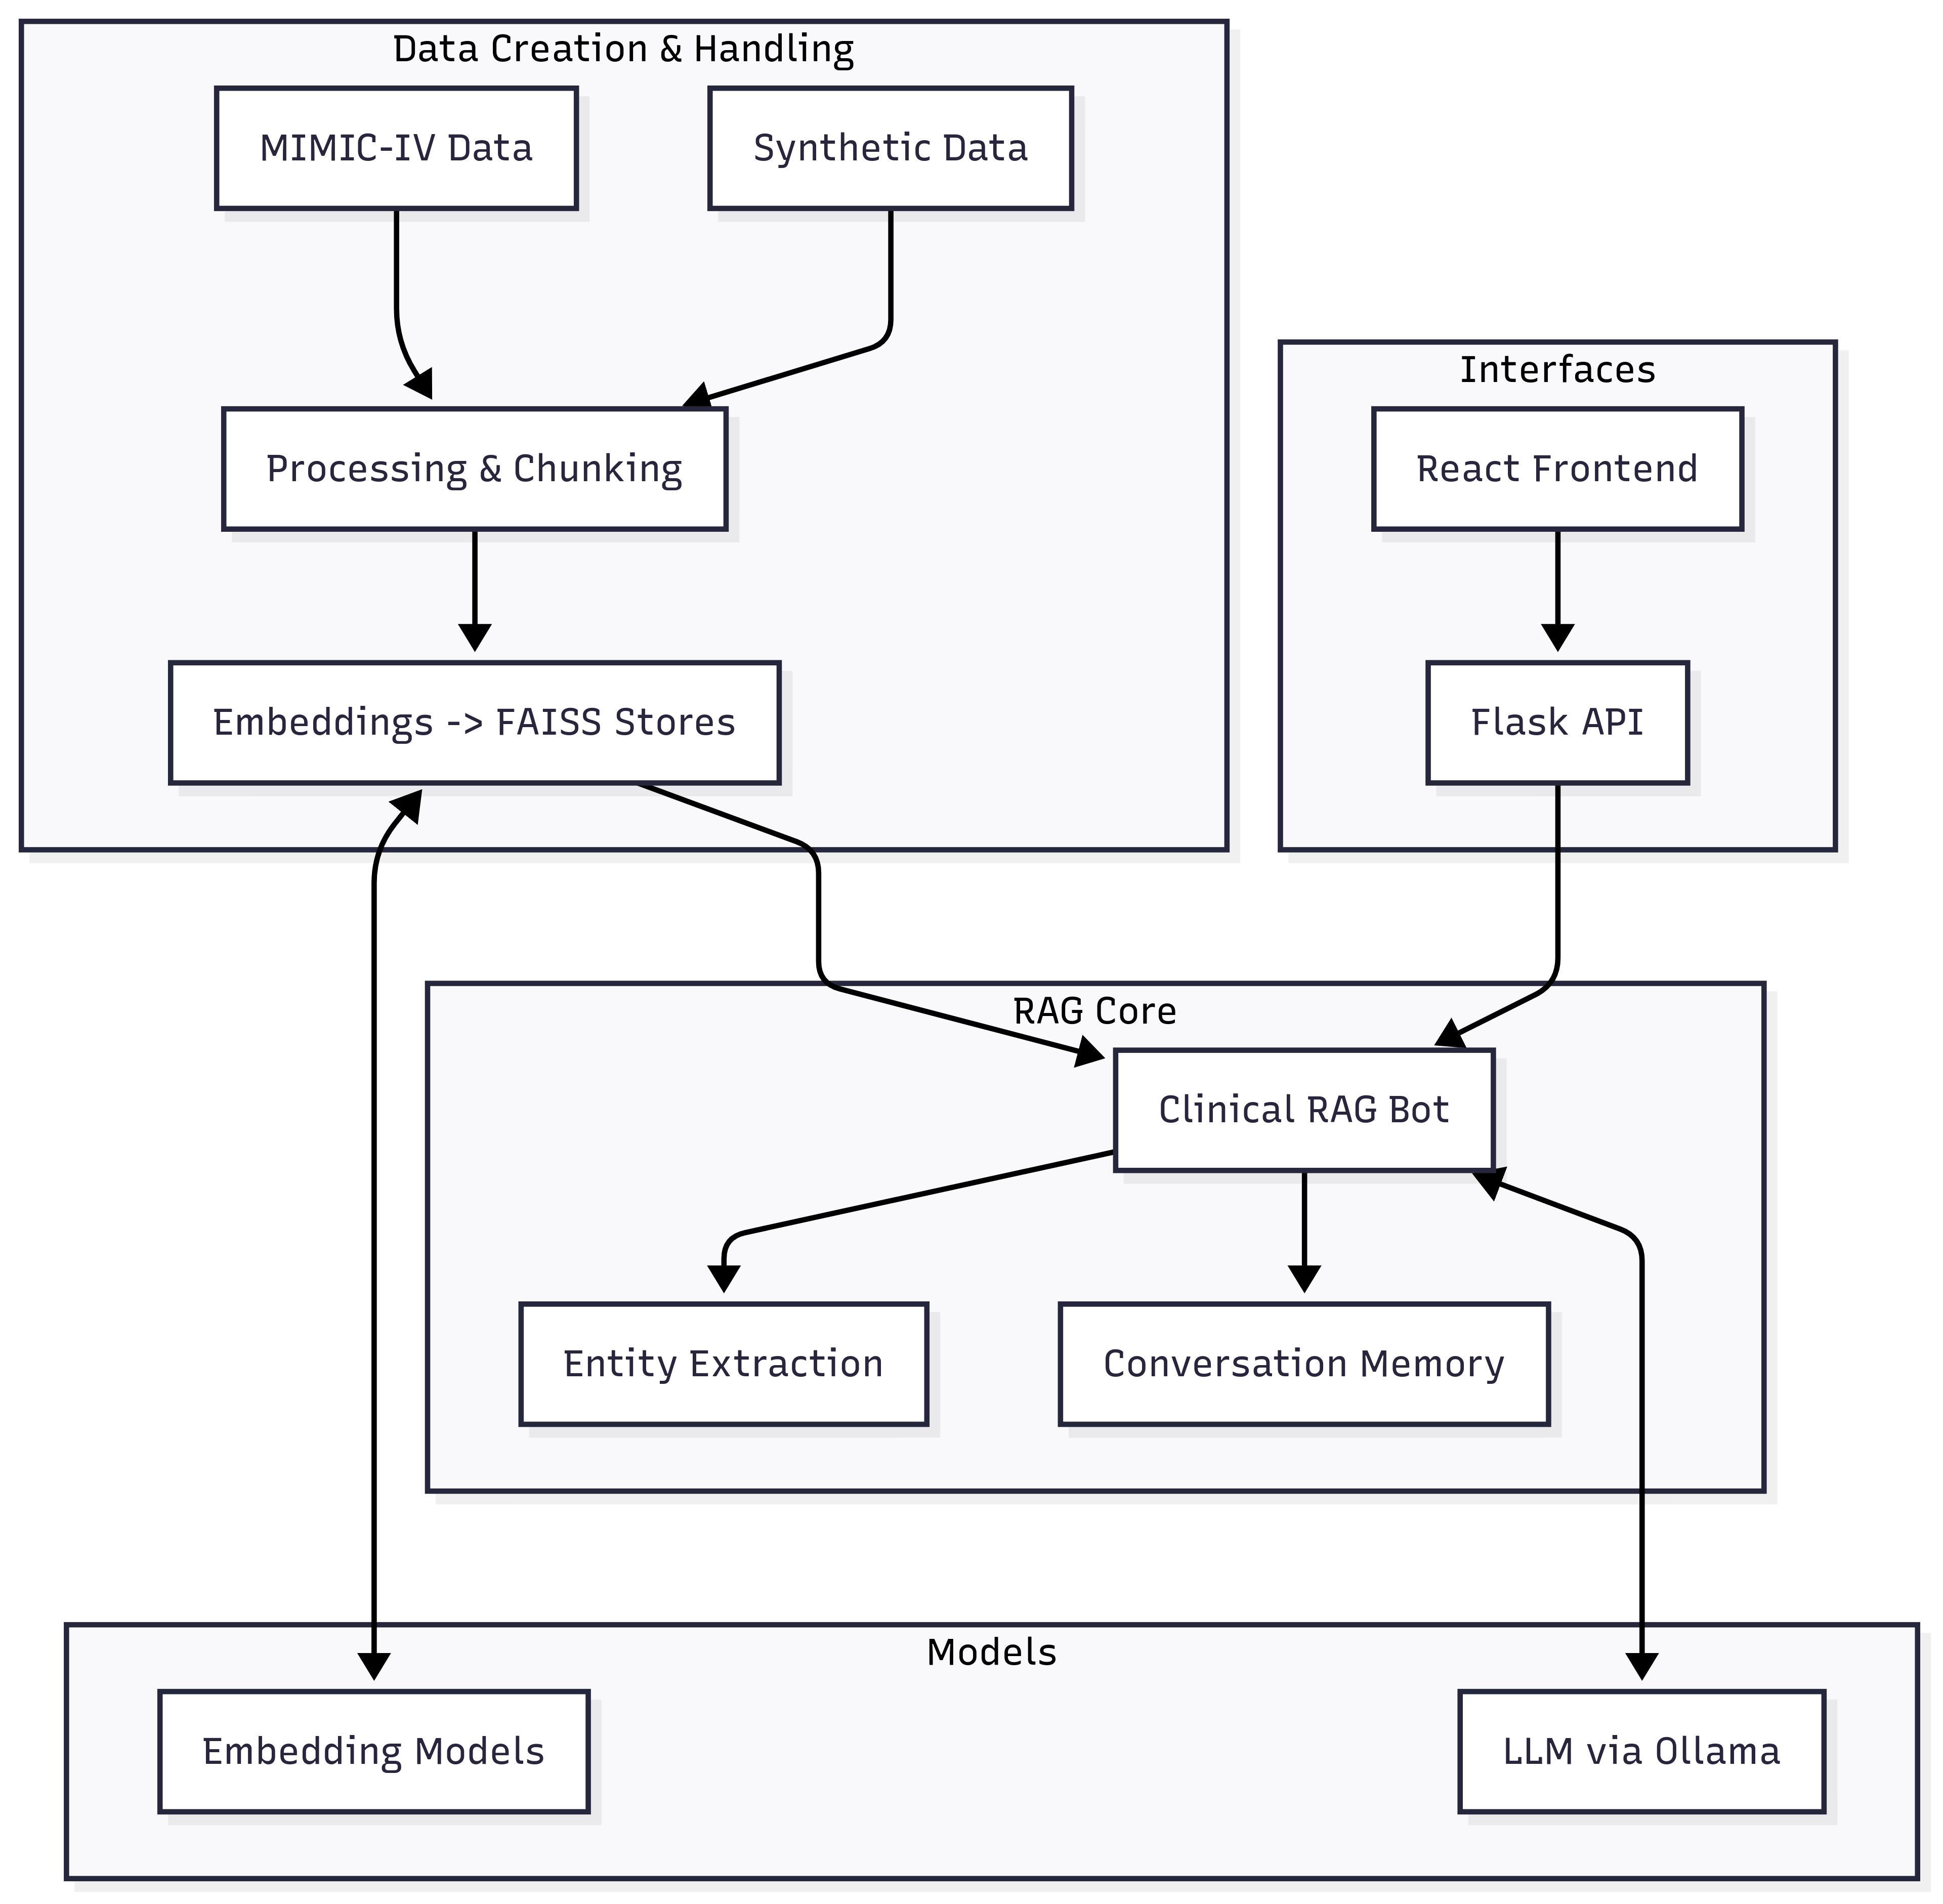
\includegraphics[width=0.95\linewidth]{chap3_methodology/images/system_archi.png}
  \caption{System architecture. Image file: \texttt{chap3_methodology/images/system_archi.png}}
  \label{fig:system_architecture}
\end{figure}


% ========================
% 3.2 Data Sources and Governance
% ========================
\section{Data Sources and Governance}

\subsection{Datasets}
\begin{itemize}
  \item Real data: MIMIC-IV sample exports are stored under \texttt{mimic\_sample\_1000/}.
  \item Synthetic data: A generator in \texttt{synthetic\_data/} produces structurally consistent, fictional clinical records for development/demo when real data are unavailable.
\end{itemize}

\noindent A data provider abstraction (\texttt{RAG\_chat\_pipeline/utils/data\_provider.py}) automatically chooses real vs. synthetic sources, preferring real MIMIC-derived exports when present.

\subsection{Ethics and Access}
Use of MIMIC-IV requires credentialed access and adherence to PhysioNet data use agreements. Public artefacts in this project are restricted to code and synthetic data. The system is intended for research/education purposes only and should not be used for clinical decision-making.

% ========================
% 3.3 Software, OS, and Runtime Environment
% ========================
\section{Software, OS, and Runtime Environment}
Experiments were executed on Microsoft Windows (user environment), Python 3.11, and React.js for the frontend.

\vspace{0.5em}
\noindent\textbf{Representative versions:}
\begin{itemize}
  \item Python: 3.11
  \item Node.js: \(\ge\) 16 (v18+ recommended)
  \item LangChain: 0.3.25; \texttt{langchain-community}: 0.3.24
  \item FAISS CPU: 1.11.0; sentence-transformers: 4.1.0
  \item Torch: 2.7.1; Transformers: 4.52.4
  \item Flask: 3.0.2; Flask-CORS: 4.0.1
  \item Ollama: 0.5.1 (models pulled locally)
\end{itemize}

% ========================
% 3.4 System Configuration
% ========================
\section{System Configuration}
Central configuration is defined in "\texttt{RAG\_chat\_pipeline/config/config.py}".

\noindent Embedding model nicknames map to HuggingFace model IDs and vector-store directories. The LLM model set is managed via Ollama. Unless otherwise specified, the session-level defaults set by \texttt{set\_models()} select \texttt{S-PubMedBert-MS-MARCO} embeddings and \texttt{deepseek-r1:1.5b} as the LLM. Alternative combinations are supported for evaluation: \texttt{all-MiniLM-L6-v2}, \texttt{multi-qa-mpnet-base-cos-v1}, \texttt{BiomedNLP-PubMedBERT}, \texttt{e5-base-v2}, \texttt{BioLORD-2023-C}, \texttt{BioBERT}, \texttt{S-PubMedBert-MedQuAD}; and LLMs such as Qwen3, Llama 3.2, Gemma 2B, Phi-3, TinyLlama).

% ========================
% 3.5 Data Processing and Document Construction
% ========================
\section{Data Processing and Document Construction}

\subsection{Preprocessing}
We prepared data with notebooks in \texttt{data\_handling/}. Sampling was performed at the admission level to produce a working subset (\texttt{mimic\_sample\_1000/}) by selecting a fixed-size random sample of \texttt{hadm\_id}s and joining the primary tables (diagnoses, procedures, labs, microbiology, prescriptions) on \texttt{hadm\_id} and \texttt{subject\_id}. This preserves cross-table coherence while controlling index size and memory footprint.

\noindent Key preprocessing steps:
\begin{enumerate}
  \item Normalise column names and types (e.g., enforce integer \texttt{hadm\_id}, \texttt{subject\_id})
  \item Map each row to a semantically labeled section: \texttt{header}, \texttt{diagnoses}, \texttt{procedures}, \texttt{labs}, \texttt{microbiology}, \texttt{prescriptions}
  \item Compose section-scoped textual records embedding key fields (codes, values/units, dates) and attach metadata
\end{enumerate}

\subsection{Chunking}
Documents are segmented into meaningful chunks optimised for clinical QA. We apply section-aware chunking before size-based splitting so that each chunk stays on the same topic (e.g., lab results grouped, diagnoses grouped). Chunk sizes of 600--900 characters with 80--150 character overlap worked well in practice for our lightweight local LLMs (balancing recall and context-window constraints). Metadata (\texttt{hadm\_id}, \texttt{subject\_id}, \texttt{section}) is preserved on every chunk to enable admission- and section-scoped retrieval.

\vspace{0.5em}
\noindent An illustrative chunking routine:
\begin{minted}[fontsize=\footnotesize, breaklines]{python}
from langchain_text_splitters import RecursiveCharacterTextSplitter

SECTION_SEPARATORS = ["\n\n", "\n", ". ", " "]

def chunk_clinical_text(text: str, chunk_size=800, chunk_overlap=120):
    splitter = RecursiveCharacterTextSplitter(
        chunk_size=chunk_size,
        chunk_overlap=chunk_overlap,
        separators=SECTION_SEPARATORS,
        is_separator_regex=False,
    )
    return splitter.split_text(text)
\end{minted}

\noindent The notebooks emit a list of \texttt{langchain.schema.Document} with \texttt{page\_content} and \texttt{metadata}, saved to \texttt{mimic\_sample\_1000/chunked\_docs.pkl} (or synthetic equivalent). These chunks are the source for vector indexing.

% ========================
% 3.6 Embeddings and Vector Stores
% ========================
\section{Embeddings and Vector Stores}

\subsection{Model Setup}
The embedding manager (\texttt{RAG\_chat\_pipeline/core/embeddings\_manager.py}) loads a SentenceTransformers model by nickname from config, caching it under \texttt{models/<model-name>/}. If not present locally, it is downloaded and saved. A \texttt{HuggingFaceEmbeddings} wrapper provides the LangChain interface.

\subsection{FAISS Indexing}
For each embedding configuration, a FAISS vector store is created from the chunked documents and saved under \texttt{vector\_stores/<store-name>/}. On startup, the system attempts to load the existing store; if missing, it builds a new one and persists both the index and the chunked corpus.

% ========================
% 3.7 RAG Pipeline and Inference
% ========================
\section{RAG Pipeline and Inference}

\subsection{RAG Contract (inputs, outputs, guardrails)}
    extbf{Inputs:} user query; optional \texttt{hadm\_id}, \texttt{subject\_id}, \texttt{section}; optional \texttt{chat\_history} (last N messages).\\
    extbf{Outputs:} answer text with inline citations; list of cited document IDs/sections; small diagnostics (retrieval mode, \(k\) used).\\
    extbf{Invariants:} ground answers strictly in retrieved content; if evidence is missing, state ``Not found in records''; always append a standard disclaimer.\\
    extbf{Constraints:} \(k \le 5\); per-section line caps in the structured context; bounded context window and per-call timeout.

\subsection{Retrieval steps (high level)}
1) Parse identifiers/section from the query and recent history (regex).\\
2) Build a candidate set using in-memory indices if hints exist; otherwise, consider the full corpus.\\
3) Rank candidates with FAISS vector similarity.\\
4) Keep top-\(k\) (default \(k=5\)).\\
5) Compact into a single structured, section-aware context (limit lines per section; prefer ICD patterns, dosages, and numeric labs).\\
6) Generate with a prompt that enforces grounding and citations.

\noindent Minimal pseudocode (illustrative):
\begin{minted}[fontsize=\footnotesize, breaklines]{python}
ids = parse_hints(query, chat_history)  # hadm_id, subject_id, section
candidates = build_candidates(ids)  # from in-memory indices or full corpus
ranked = faiss_rank(candidates, query)
topk = ranked[: min(k, 5)]
context = make_structured_context(topk)  # section-aware, line-capped
answer = llm_answer(query, context, prompt=CLINICAL_PROMPT)
return answer
\end{minted}

\subsection{Retriever}
Given a query, the pipeline first attempts metadata-constrained retrieval when a \texttt{hadm\_id}, \texttt{subject\_id}, or \texttt{section} is available. Efficient in-memory indices (built at bot initialisation) map identifiers and sections to candidate document IDs, reducing the search space before semantic ranking. Otherwise, a global FAISS similarity search is performed.

\vspace{0.5em}
\noindent At initialisation, the bot builds light-weight Python indices for fast filtering:
\begin{minted}[fontsize=\footnotesize, breaklines]{python}
from collections import defaultdict

self.hadm_id_index = defaultdict(list)
self.subject_id_index = defaultdict(list)
self.section_index = defaultdict(list)
self.hadm_section_index = defaultdict(list)

for i, doc in enumerate(self.chunked_docs):
    hadm = doc.metadata.get("hadm_id")
    sec = str(doc.metadata.get("section", "")).lower()
    if hadm is not None:
        try:
            hadm_i = int(hadm)
            self.hadm_id_index[hadm_i].append(i)
            if sec:
                self.hadm_section_index[(hadm_i, sec)].append(i)
        except ValueError:
            pass
    if sec:
        self.section_index[sec].append(i)
\end{minted}

\noindent When a \texttt{hadm\_id} or \texttt{section} is present, only the corresponding candidate set is ranked semantically.

\subsection{Context Construction}
Top-$k$ (default \(k=5\), bounded for performance) documents are semantically ranked. For efficiency and to improve answer formatting, the system extracts concise, section-aware snippets (diagnoses, procedures, labs, prescriptions, microbiology, header) and composes a single structured context document passed to the LLM. Rules favour lines with section-specific keywords and patterns (e.g., ICD codes, dosages, numeric lab values/units) while limiting per-section lines to keep within context windows.

\subsection{LLM Answering}
Answers are generated using an Ollama-hosted model (default DeepSeek-R1 1.5B) through LangChain's \texttt{create\_stuff\_documents\_chain}, with a prompt that enforces the guardrails below.

\noindent \textbf{Prompt guardrails:}
\begin{itemize}
  \item Cite sources inline and include codes/values/units/dates when present
  \item If evidence is missing, say so; do not guess
  \item Respect admission/section scope when provided
  \item Always append the standard disclaimer
\end{itemize}

\subsection{Entity Extraction and Conversational Context}
A deterministic regex-based extractor (\texttt{helper/entity\_extraction.py}) identifies \texttt{hadm\_id}, \texttt{subject\_id}, and \texttt{section} hints from the current query and recent chat messages. For follow-ups, an LLM-powered rephrasing step condenses the question into a standalone form while preserving identifiers. Chat history is truncated to a configurable maximum (\textbf{60 messages}; see \texttt{MAX\_CHAT\_HISTORY} in config) to control context length.

\subsection{RAG Core Emphasis and Design Evolution}
The initial blueprint used a straightforward vector index + chat engine with strict context mode:
\begin{minted}[fontsize=\footnotesize, breaklines]{python}
from llama_index.core import VectorStoreIndex, SimpleDirectoryReader
from llama_index.embeddings.ollama import OllamaEmbedding
from llama_index.llms.ollama import Ollama

docs = SimpleDirectoryReader("./parsed_emails").load_data()
embed_model = OllamaEmbedding(model_name="nomic-embed-text")
llm = Ollama(model="llama3.2")

index = VectorStoreIndex.from_documents(docs, embed_model=embed_model)
chat_engine = index.as_chat_engine(
    llm=llm,
    chat_mode="context",
    verbose=True
)
response = chat_engine.chat("There is package mentioned for spaghetti code")
\end{minted}

We attempted a two-step pipeline (LLM judges chunk relevance, then answers), but lightweight local models had small context windows and were unreliable as rankers. The reliable fix was a \textbf{custom retriever}: extract \texttt{hadm\_id}/\texttt{subject\_id}/\texttt{section} via regex/patterns, filter candidates with in-memory indices, reduce content by meaning, then pass only the top snippets to the LLM. The core search is:
\begin{minted}[fontsize=\footnotesize, breaklines]{python}
candidate = self._filter_candidate_documents(hadm_id, subject_id, section, limit=20)
if candidate is None:
    retrieved = self.vectorstore.similarity_search(question, k=min(k, 20))
else:
    retrieved = self._semantic_search_on_docs(candidate, question, k=min(k, 5))
structured = self._extract_clinical_content(retrieved)
prompt = self._create_clinical_prompt(hadm_id, subject_id)
chain = create_stuff_documents_chain(self.llm, prompt)
answer = safe_llm_invoke(chain, {"input": question, "context": [Document(page_content=structured)]})
\end{minted}

% Consolidated hallucination mitigation earlier; avoid repetition here.

% ========================
% 3.8 Interfaces
% ========================
\section{Interfaces}

\subsection{API}
A Flask service in \texttt{api/app.py} exposes endpoints:
\begin{itemize}
  \item \texttt{POST /api/chat}: process a chat message and optional history
  \item \texttt{GET /api/models}: list available embedding models and vector stores
  \item Static serving: production build of the React app
\end{itemize}

\noindent \textbf{Chat endpoint contract (summary):}
\begin{itemize}
  \item Request: \{\texttt{query: str}, optional \texttt{hadm\_id}, \texttt{subject\_id}, \texttt{section}, optional \texttt{history: [\{role, content\}] }\}
  \item Response: \{\texttt{answer: str}, \texttt{citations: [\{doc\_id, section\}]}, \texttt{diagnostics: \{mode, k\}}\}
\end{itemize}

\subsection{Frontend}
A React UI (\texttt{frontend/}) provides a chat interface, model introspection, and sample query suggestions sourced from the data provider.

\subsection{CLI}
\texttt{cli\_chat.py} offers an interactive console with session logging and history management.

% ========================
% 3.9 Challenges and Mitigations
% ========================
\section{Challenges and Mitigations}
    extbf{Risk: medical hallucinations and sensitive data.} Early versions retrieved globally and over-supplied context, which could produce made-up details. Mitigations:
\begin{itemize}
  \item Admission-/section-scoped retrieval via in-memory indices
  \item Deterministic entity extraction (regex) to avoid LLM-based unexpected settings changes
  \item Structured snippet extraction with section rules
  \item Post-processing to enforce disclaimers and fix citations
\end{itemize}

\noindent Replacing the two-step LLM-as-ranker approach with the custom retriever + semantic re-ranking significantly improved factual grounding on lightweight local models.

\noindent \textbf{Failure modes and fallbacks:}
\begin{itemize}
  \item Missing hints (no IDs/section) \textrightarrow{} use global search
  \item Empty candidate set \textrightarrow{} fall back to global k-NN
  \item FAISS store missing at startup \textrightarrow{} rebuild once, then cache
  \item Timeout or partial retrieval \textrightarrow{} return a safe message without guessing
\end{itemize}

% ========================
% 3.10 Evaluation Protocol
% ========================
\section{Evaluation Protocol}
We provide only a brief overview here; detailed metrics and comparisons are in Results. The evaluator generates category-specific gold questions and computes pass/fail and summary statistics per model combination. We validate against structured signals (ICD patterns, dosages, units) and measure retrieval latency; full scoring details are in Results.

\subsection{Gold Questions and Categories}
Gold questions are created from available records (diagnoses, procedures, labs, etc.) with associated \texttt{hadm\_id}s when applicable. Full evaluation outcomes are reported in Results.

% ========================
% 3.11 Modularity and Extensibility
% ========================
\section{Modularity and Extensibility}
The system is modular: configuration (\texttt{config/}), core RAG components (\texttt{core/}), helpers, utilities, API, and frontend are decoupled. Models are selectable at runtime (\texttt{set\_models()}), and vector stores are tied to embeddings, enabling comparison tests.

% ========================
% 3.12 Reproducibility
% ========================
\section{Reproducibility}

\subsection{Environment Setup}
\begin{enumerate}
  \item Create Python 3.11 env: \texttt{pip install -e .}
  \item Install frontend deps: \texttt{cd frontend \&\& npm install}
  \item Install Ollama and pull models: \texttt{deepseek-r1:1.5b}
\end{enumerate}

\subsection{Data Preparation}
\begin{itemize}
  \item Real data: Place MIMIC-IV exports under \texttt{mimic\_sample\_1000/}, run \texttt{creating\_docs.ipynb}
  \item Synthetic data: Run \texttt{synthetic\_data\_generator.py}
\end{itemize}

\subsection{Running and Evaluation}
\begin{itemize}
  \item API: \texttt{python api/app.py}
  \item UI: \texttt{cd frontend; npm start}
  \item CLI: \texttt{python cli\_chat.py chat}
  \item Quick eval: \texttt{python -m benchmarks.model\_evaluation\_runner single ms-marco deepseek short}
  \item Full comp: \texttt{python -m benchmarks.model\_evaluation\_runner all full}
\end{itemize}

% ========================
% 3.13 Quality Assurance
% ========================
\section{Quality Assurance and Performance}
The chatbot uses in-memory indices for fast filtering and embedding caching. Retrieval sets are capped for latency control. Post-processing normalises outputs.

\noindent \textbf{Deterministic behaviour and caching:} model versions are pinned; random seeds set where applicable; embeddings cached on disk; \(k\) and per-section limits fixed; chat history bounded.

% ========================
% 3.14 Limitations
% ========================
\section{Limitations}
We evaluate on limited MIMIC/synthetic data. Local LLMs (1-4B params) balance privacy/cost but may underperform large models. Results depend on embeddings, chunking, and prompting.

% ========================
% 3.15 Summary
% ========================
\section{Summary}
The methodology provides an end-to-end, reproducible pipeline from MIMIC-compatible data to a clinical RAG system. All components are parameterised to support comparison tests.

    \chapter{Results \& Discussion}
\label{chap:results}

\noindent This chapter reports the outcomes of our Clinical RAG evaluation and discusses the key findings. We reiterate the study aims: to quantify how different embedding models and small LLMs affect end-to-end retrieval-augmented answering quality, speed, and safety on a clinical QA set.

\section{Experiment Overview}
\begin{itemize}
  \item Total experiments: 54 runs (9 embedding models \(\times\) 6 LLMs).
  \item Embeddings: ms-marco, multi-qa, mini-lm, biomedbert, mpnet-v2, e5-base, BioLORD, BioBERT, MedQuAD.
  \item LLMs: deepseek, qwen, llama, gemma, phi3, tinyllama.
  \item Per-run questions: 20; metrics include pass rate, average score (primary), search time, documents found; efficiency/safety include throughput (QPM), disclaimer and hallucination rates.
\end{itemize}

\section{Overall Performance}
Aggregate results across all 54 runs show:
\begin{itemize}
  \item Average pass rate: 89.6\%.
  \item Average score: 0.706.
  \item Average search time: 98.77s.
\end{itemize}

Best-performing configurations:
\begin{itemize}
  \item Highest overall score: BioBERT + phi3 (avg. score 0.770, 100\% pass rate).
  \item Fastest: e5-base + deepseek (avg. search time 53.28s, avg. score 0.640).
\end{itemize}

\section{Comparison Heatmap}
Figure~\ref{fig:heatmap_avg_score} provides a model-by-model comparison heatmap (average score). An interactive version is available as HTML in the results folder.

\begin{figure}[h]
  \centering
  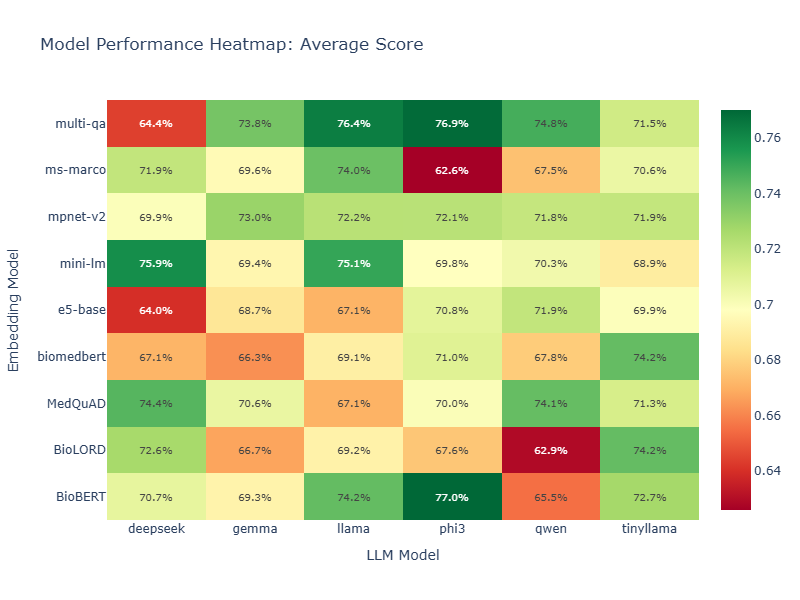
\includegraphics[width=\textwidth]{chap4_results/images/heatmap_average_score.png}
  \caption{Model comparison heatmap by average score.}
  \label{fig:heatmap_avg_score}
\end{figure}

\section{Top-Performing Configurations}
Table~\ref{tab:top_configs} reports the top configurations by average score. We report pass rate and average search time to capture effectiveness and efficiency trade-offs.

\newcolumntype{P}[1]{>{\centering\arraybackslash}p{#1}}
\newcolumntype{Y}{>{\centering\arraybackslash}X}

\begin{table}[h]
\centering
\begin{footnotesize}
\renewcommand\arraystretch{0.95}
\begin{tabularx}{\textwidth}{l l P{1.6cm} P{1.6cm} P{1.8cm}}
  \toprule
  Embedding & LLM & Pass rate & Avg. score & Avg. search time (s) \\
  \midrule
  BioBERT & phi3 & 100\% & 0.770 & 67.70 \\
  multi-qa & llama & 95\% & 0.764 & 61.20 \\
  multi-qa & phi3 & 95\% & 0.769 & 70.77 \\
  mini-lm & deepseek & 95\% & 0.759 & 326.02 \\
  mini-lm & llama & 100\% & 0.751 & 56.50 \\
  MedQuAD & deepseek & 90\% & 0.744 & 355.67 \\
  BioBERT & llama & 90\% & 0.742 & 82.48 \\
  BioLORD & tinyllama & 95\% & 0.742 & 73.44 \\
  biomedbert & tinyllama & 95\% & 0.742 & 355.25 \\
  MedQuAD & qwen & 95\% & 0.741 & 69.12 \\
  \bottomrule
\end{tabularx}
\end{footnotesize}
\caption{Top-performing configurations by average score.}
\label{tab:top_configs}
\end{table}

\paragraph{Observations.} The best average scores are achieved by BioBERT + phi3 and multi-qa + phi3/llama. MiniLM pairs (mini-lm + llama/deepseek) are strong with excellent pass rates; however, mini-lm + deepseek exhibits much longer search time, suggesting backend or retrieval interaction overhead. MedQuAD-based embeddings produce competitive average scores but at times with slower end-to-end latency.

\section{Efficiency and Safety}
We summarize representative efficiency and safety outcomes in Table~\ref{tab:efficiency_safety}. Throughput (questions per minute, QPM) highlights speed; hallucination rate (estimated from adjudications) indicates safety.

\begin{table}[h]
\centering
\begin{footnotesize}
\renewcommand\arraystretch{0.95}
\begin{tabularx}{0.9\textwidth}{l l P{1.3cm} P{1.4cm} P{1.5cm}}
  \toprule
  Embedding & LLM & QPM & Avg. score & Hallucination \\
  \midrule
  e5-base & deepseek & 1.122 & 0.640 & 0.40 \\
  mini-lm & qwen & 1.100 & 0.703 & 0.30 \\
  mini-lm & llama & 1.059 & 0.751 & 0.15 \\
  MedQuAD & deepseek & 0.169 & 0.744 & 0.10 \\
  \bottomrule
\end{tabularx}
\label{tab:efficiency_safety}
  \bottomrule
\end{tabularx}
\end{footnotesize}
\caption{Efficiency and safety metrics.}
\label{tab:efficiency_safety}
\end{table}

\paragraph{Trade-offs.} The fastest pipeline (e5-base + deepseek) sacrifices some answer quality relative to the top-scoring setups. Mini-lm + llama offers an appealing balance: perfect pass rate, good average score, high throughput, and low hallucination. The safest configuration by hallucination rate (MedQuAD + deepseek) is slower; this may reflect conservative generation behavior or heavier retrieval.

\section{Discussion}
Overall, average score is a more discriminative primary KPI than pass rate, revealing nuanced differences among competitive pairs. Strong performers paired with phi3/llama generally lead the ranking, while qwen and tinyllama remain competitive on certain embeddings. Category analysis indicates substantial headroom for structured clinical facts (labs, microbiology, prescriptions); targeted retrieval improvements (e.g., table-aware chunking, ontology-linked indices) and instruction-tuned prompts for evidence citation are likely to close this gap. Finally, efficiency/safety analysis underscores practical deployment choices: mini-lm + llama emerges as a well-balanced default; BioBERT + phi3 is optimal for peak accuracy; and e5-base + deepseek can serve latency-sensitive workflows when moderate quality is acceptable.

\section*{Artifacts}
The following artifacts are available in the results folder for reproducibility and further analysis: heatmap PNG and interactive HTML, the consolidated CSVs (results\_dataframe.csv, per\_question\_results.csv), efficiency/safety metrics (run\_efficiency\_and\_safety.csv), and the summary report (summary\_report.md).

% -----------------------------------------
% Evaluation methodology and metric rationale
% -----------------------------------------
\section{Evaluation Methodology and Metrics}
This section explains each evaluation we report, why it matters for clinical RAG, and how to interpret it.

\subsection{Average Score (primary KPI)}
The average score is a normalized 0--1 rating aggregated across questions. It reflects overall answer quality by combining rubric criteria such as factual correctness, sufficiency of evidence, and clinical appropriateness. We prioritize this as the primary KPI because it is sensitive to partial improvements that pass/fail metrics may miss and aligns with qualitative judgments of clinical usefulness.

\subsection{Pass Rate}
Pass rate is the proportion of questions meeting a minimum threshold (``acceptable'' grade). It is intuitive and robust, enabling quick comparisons of reliability. However, it is coarse; it does not distinguish between barely passing and very strong answers, so we pair it with the average score.

\subsection{Factual Accuracy and Performance Subscores}
Where available, we report separate subscores (e.g., factual accuracy, performance/presentation). Factual accuracy captures grounding to retrieved evidence and correctness of clinical facts; performance captures clarity, organization, and adherence to instructions (e.g., concise rationale, citations). Separating these clarifies whether errors arise from retrieval grounding or from generation quality.

\subsection{Latency and Throughput}
Average search time (seconds) measures end-to-end latency per question, dominated by retrieval plus model generation. Throughput (questions per minute, QPM) summarises system capacity under load. Clinical settings often require timely responses; we therefore report both and examine speed/quality trade-offs (e.g., e5-base + deepseek is fastest but with lower average score than top-accuracy pairs).

\subsection{Retrieval Coverage}
Average documents found provides a coarse proxy for retrieval depth and coverage. Too few documents may under-support grounding; too many may add noise and increase latency. Configurations that maintain strong scores with modest document counts indicate efficient, focused retrieval.

\subsection{Safety Indicators}
Hallucination rate approximates the frequency of unsupported or factually incorrect statements. Lower is safer. Disclaimer rate captures frequency of safety/compliance disclaimers; in clinical RAG, some disclaimers are appropriate, but overuse can reduce usefulness. We interpret these together with quality metrics to identify safe and useful operating points.

\subsection{Per-Question Analysis}
Per-question results (in \texttt{per\_question\_results.csv}) enable drill-down into failure modes (e.g., missing lab values, incorrect medication dosages) and success cases. These analyses inform targeted improvements (schema-aware chunking, ontology-linked retrieval, citation prompting).

% A compact summary table for quick reference
\begin{table}[h]
\centering
\begin{footnotesize}
\renewcommand\arraystretch{0.95}
\begin{tabular}{l p{6.2cm} p{6.2cm}}
  \toprule
  Metric & What it measures & Why it matters in clinical RAG \\
  \midrule
  Average score & Overall answer quality (0--1) across questions & Sensitive to partial improvements; aligns with perceived clinical usefulness \\
  Pass rate & Fraction of answers meeting an acceptability threshold & Simple reliability signal; complements average score \\
  Factual accuracy & Grounding and correctness of clinical facts & Directly tied to patient safety and evidence use \\
  Performance/presentation & Structure, clarity, instruction adherence & Affects readability, clinician trust, and efficiency \\
  Search time & Latency per question (s) & Practical responsiveness for clinical workflows \\
  Throughput (QPM) & Questions processed per minute & Capacity planning and cost/performance trade-offs \\
  Documents found & Retrieval depth/coverage proxy & Balances evidence sufficiency vs. noise/latency \\
  Hallucination rate & Unsupported/incorrect content frequency & Safety and risk mitigation \\
  Disclaimer rate & Frequency of safety disclaimers & Compliance vs. usefulness balance \\
  \bottomrule
\end{tabular}
\end{footnotesize}
\caption{Summary of evaluation metrics and their importance in clinical RAG.}
\label{tab:metrics_summary}
\end{table}

% Auto-generated comprehensive tables
\section{Comprehensive Tables}
To aid reproducibility, we include the full set of runs and category-wise averages generated from the consolidated CSVs.

\subsection{All 54 Runs (sorted by average score)}
% Note: Replace this with actual table content when available
\begin{center}
\begin{footnotesize}
\renewcommand\arraystretch{0.95}
% Auto-generated from results_dataframe.csv and run_efficiency_and_safety.csv
\begin{tabularx}{\textwidth}{l l c c c c}
  \toprule
  Embedding & LLM & Pass rate (\%) & Avg. score & Search time (s) & QPM \
  \midrule
  BioBERT & phi3 & 100.0 & 0.770 & 67.70 & 0.884 \
  multi-qa & phi3 & 95.0 & 0.769 & 70.77 & 0.845 \
  multi-qa & llama & 95.0 & 0.764 & 61.20 & 0.978 \
  mini-lm & deepseek & 95.0 & 0.759 & 326.02 & 0.184 \
  mini-lm & llama & 100.0 & 0.751 & 56.50 & 1.059 \
  multi-qa & qwen & 95.0 & 0.748 & 72.68 & 0.823 \
  MedQuAD & deepseek & 90.0 & 0.744 & 355.67 & 0.169 \
  biomedbert & tinyllama & 95.0 & 0.742 & 355.25 & 0.169 \
  BioLORD & tinyllama & 95.0 & 0.742 & 73.44 & 0.815 \
  BioBERT & llama & 90.0 & 0.742 & 82.48 & 0.725 \
  MedQuAD & qwen & 95.0 & 0.741 & 69.12 & 0.865 \
  ms-marco & llama & 90.0 & 0.740 & 72.60 & 0.822 \
  multi-qa & gemma & 90.0 & 0.738 & 77.55 & 0.772 \
  mpnet-v2 & gemma & 100.0 & 0.730 & 74.35 & 0.805 \
  BioBERT & tinyllama & 95.0 & 0.727 & 69.87 & 0.856 \
  BioLORD & deepseek & 90.0 & 0.726 & 65.96 & 0.907 \
  mpnet-v2 & llama & 85.0 & 0.722 & 69.29 & 0.863 \
  mpnet-v2 & phi3 & 90.0 & 0.721 & 61.62 & 0.971 \
  e5-base & qwen & 100.0 & 0.719 & 66.99 & 0.893 \
  ms-marco & deepseek & 95.0 & 0.719 & 71.14 & 0.841 \
  mpnet-v2 & tinyllama & 95.0 & 0.719 & 79.34 & 0.754 \
  mpnet-v2 & qwen & 100.0 & 0.718 & 65.52 & 0.913 \
  multi-qa & tinyllama & 85.0 & 0.715 & 70.61 & 0.847 \
  MedQuAD & tinyllama & 90.0 & 0.713 & 67.55 & 0.885 \
  biomedbert & phi3 & 90.0 & 0.710 & 69.87 & 0.856 \
  e5-base & phi3 & 100.0 & 0.708 & 60.60 & 0.986 \
  BioBERT & deepseek & 90.0 & 0.707 & 69.83 & 0.857 \
  MedQuAD & gemma & 85.0 & 0.706 & 70.92 & 0.843 \
  ms-marco & tinyllama & 80.0 & 0.706 & 62.50 & 0.957 \
  mini-lm & qwen & 90.0 & 0.703 & 54.39 & 1.100 \
  MedQuAD & phi3 & 90.0 & 0.700 & 68.14 & 0.878 \
  e5-base & tinyllama & 95.0 & 0.699 & 353.18 & 0.170 \
  mpnet-v2 & deepseek & 90.0 & 0.699 & 67.78 & 0.883 \
  mini-lm & phi3 & 85.0 & 0.698 & 353.36 & 0.170 \
  ms-marco & gemma & 90.0 & 0.696 & 61.34 & 0.975 \
  mini-lm & gemma & 100.0 & 0.694 & 61.13 & 0.979 \
  BioBERT & gemma & 95.0 & 0.693 & 67.09 & 0.892 \
  BioLORD & llama & 90.0 & 0.692 & 70.04 & 0.854 \
  biomedbert & llama & 85.0 & 0.691 & 71.43 & 0.838 \
  mini-lm & tinyllama & 90.0 & 0.689 & 67.78 & 0.883 \
  e5-base & gemma & 90.0 & 0.687 & 65.57 & 0.912 \
  biomedbert & qwen & 80.0 & 0.678 & 58.61 & 1.020 \
  BioLORD & phi3 & 85.0 & 0.676 & 69.92 & 0.856 \
  ms-marco & qwen & 85.0 & 0.675 & 66.41 & 0.901 \
  e5-base & llama & 85.0 & 0.671 & 63.97 & 0.935 \
  biomedbert & deepseek & 80.0 & 0.671 & 359.51 & 0.167 \
  MedQuAD & llama & 80.0 & 0.671 & 63.43 & 0.943 \
  BioLORD & gemma & 85.0 & 0.667 & 66.66 & 0.897 \
  biomedbert & gemma & 85.0 & 0.663 & 69.77 & 0.858 \
  BioBERT & qwen & 80.0 & 0.655 & 62.70 & 0.954 \
  multi-qa & deepseek & 75.0 & 0.644 & 70.20 & 0.852 \
  e5-base & deepseek & 80.0 & 0.640 & 53.28 & 1.122 \
  BioLORD & qwen & 75.0 & 0.629 & 66.17 & 0.904 \
  ms-marco & phi3 & 80.0 & 0.626 & 64.61 & 0.926 \
  \bottomrule
\end{tabularx}
\end{footnotesize}
\end{center}


\section{Additional Figures}
\begin{figure}[h]
  \centering
  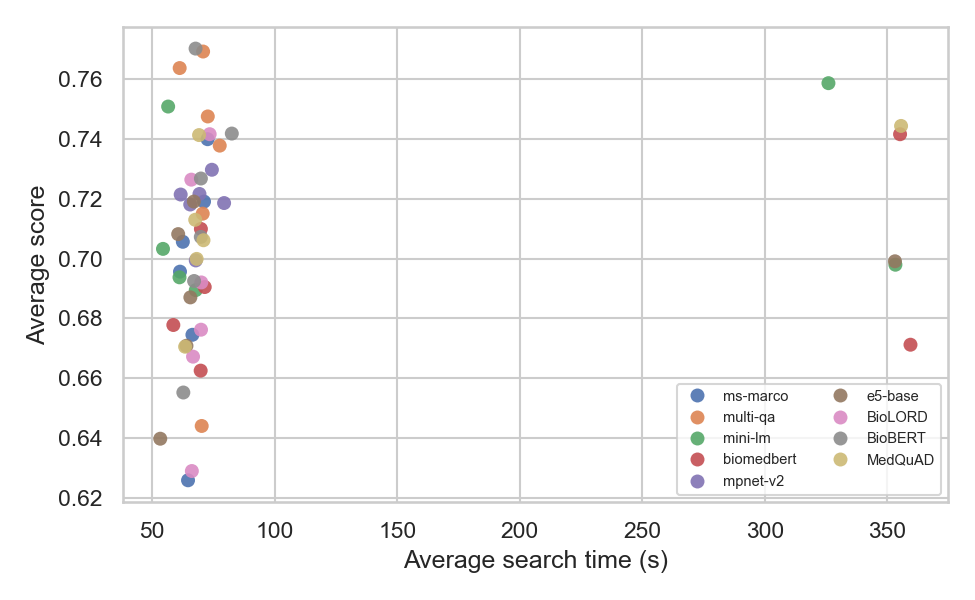
\includegraphics[width=\textwidth]{chap4_results/images/time_vs_score.png}
  \caption{Average score vs. average search time across all runs. Lower time and higher score are better.}
  \label{fig:time_vs_score}
\end{figure}

\begin{figure}[h]
  \centering
  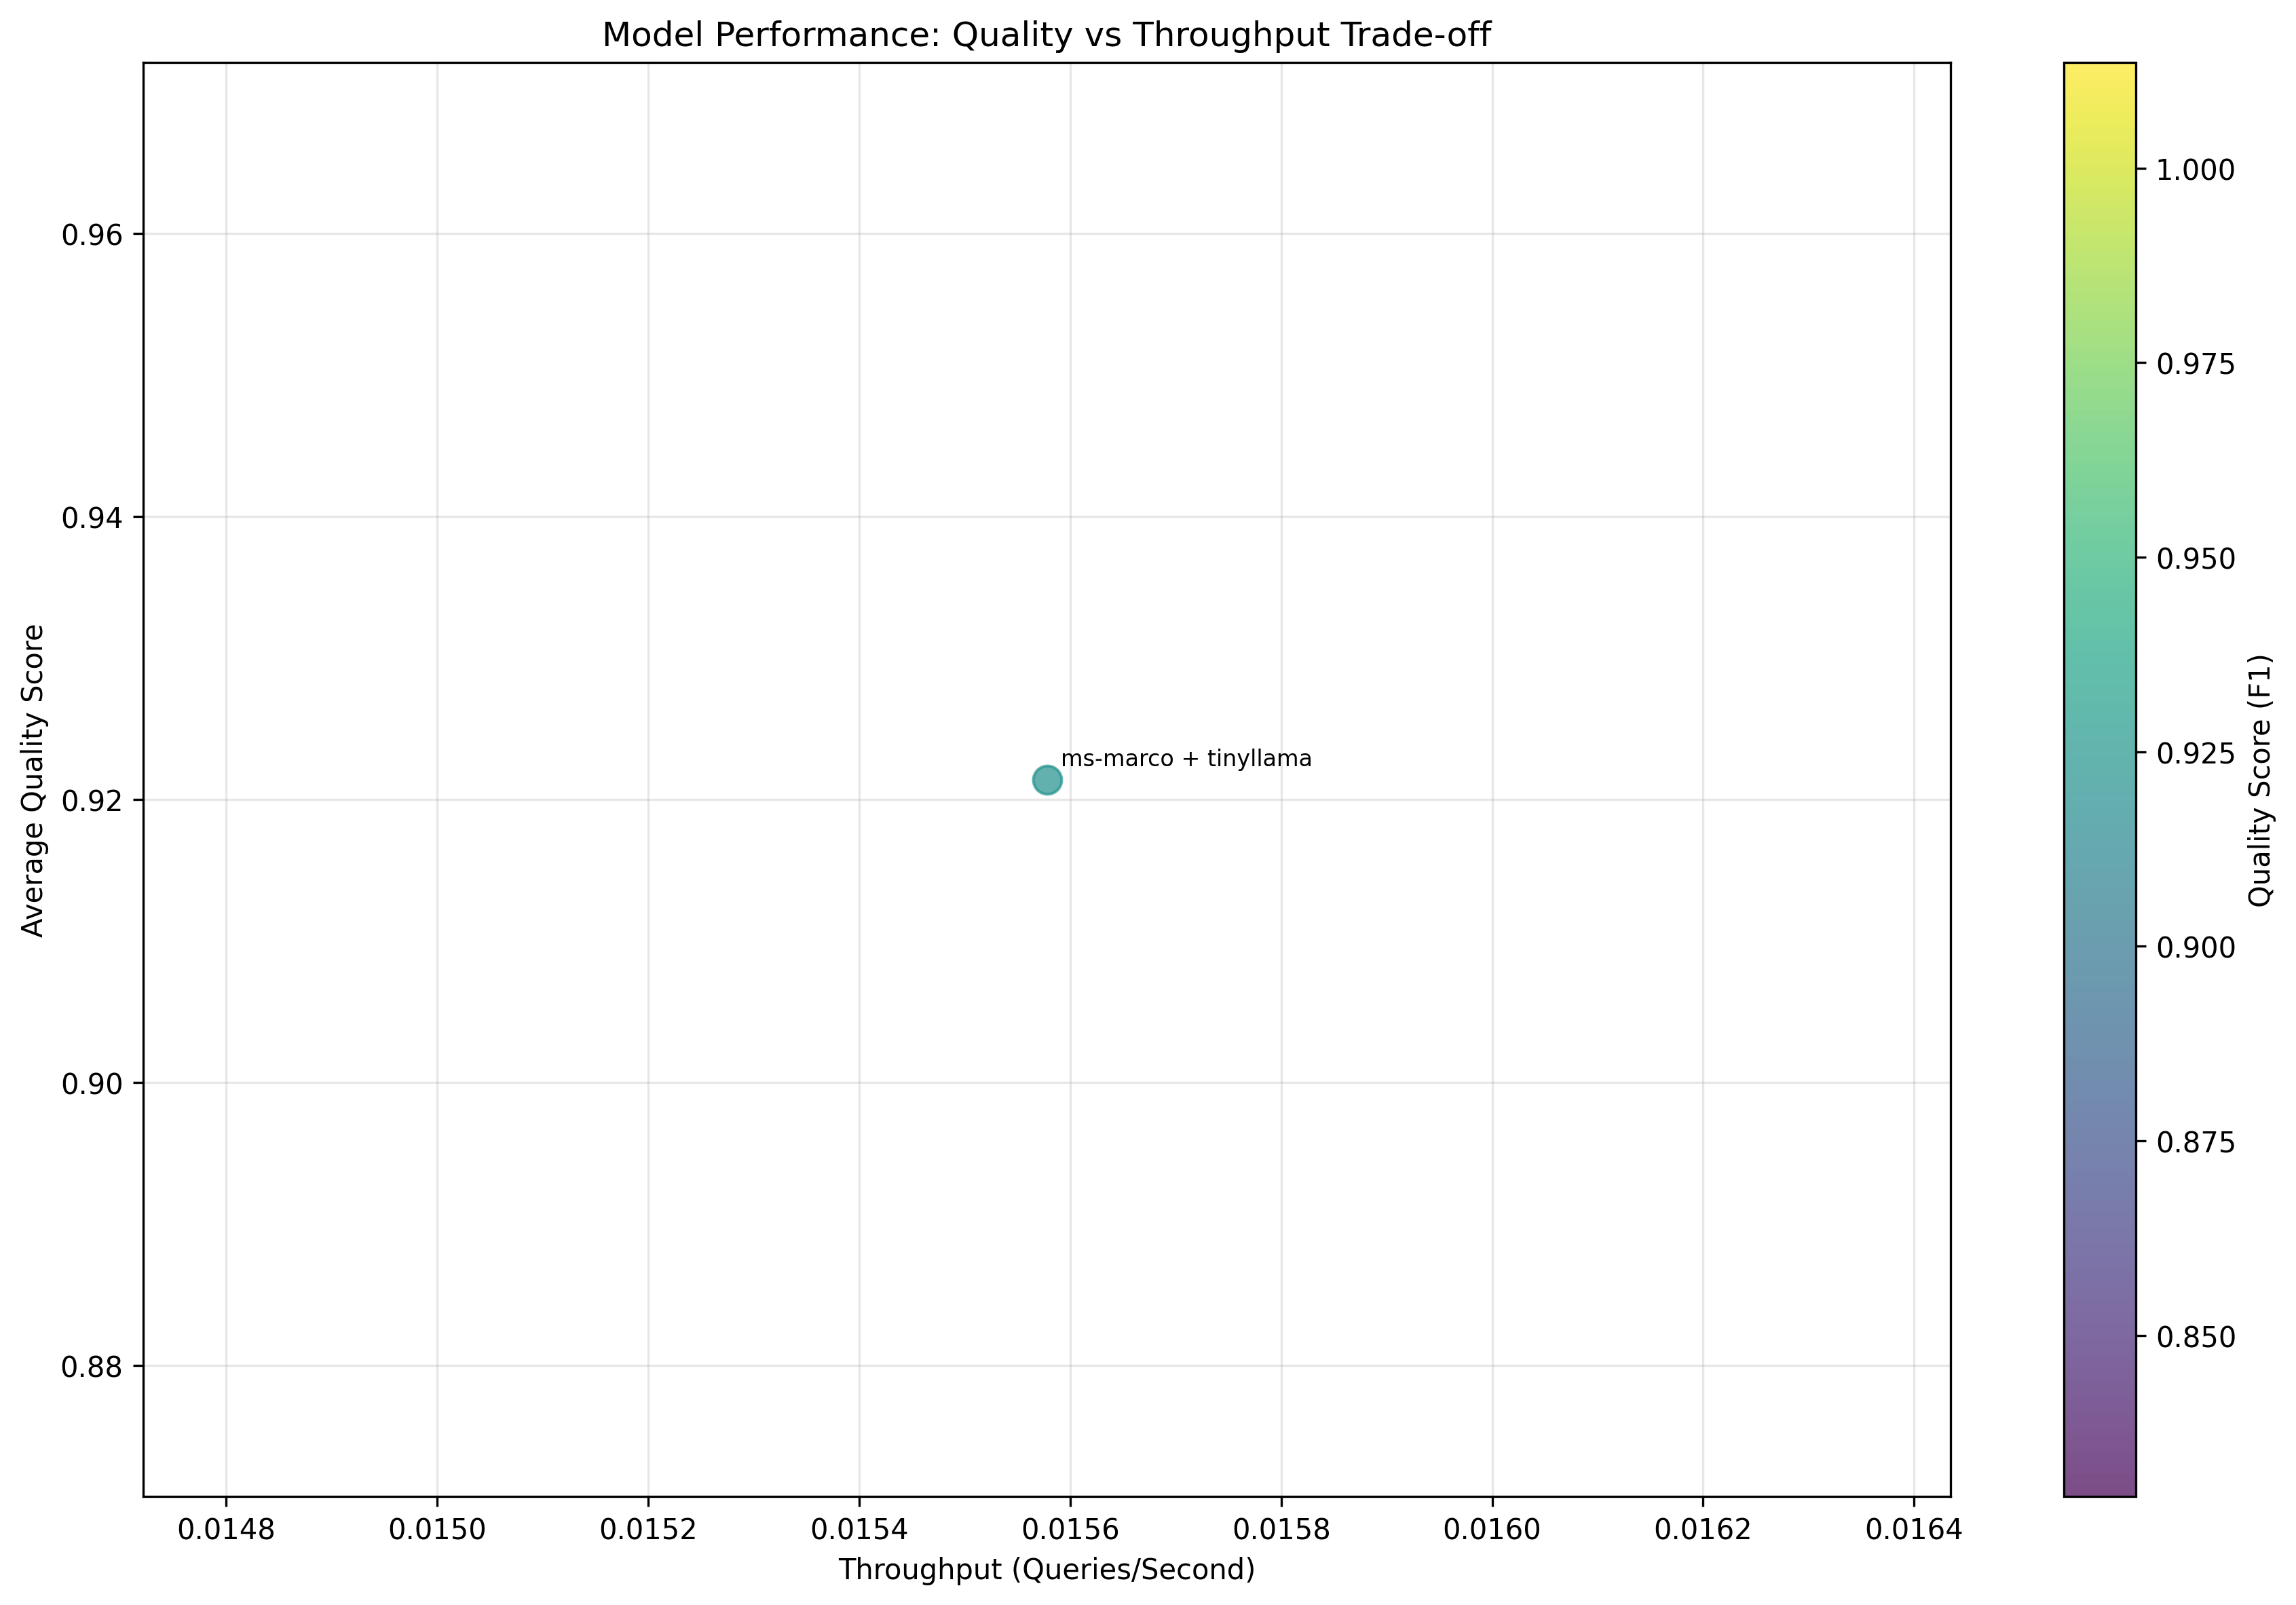
\includegraphics[width=\textwidth]{chap4_results/images/quality_vs_throughput.png}
  \caption{Average score vs. throughput (QPM). Useful to identify speed-quality efficient frontiers.}
  \label{fig:quality_vs_throughput}
\end{figure}

\begin{figure}[h]
  \centering
  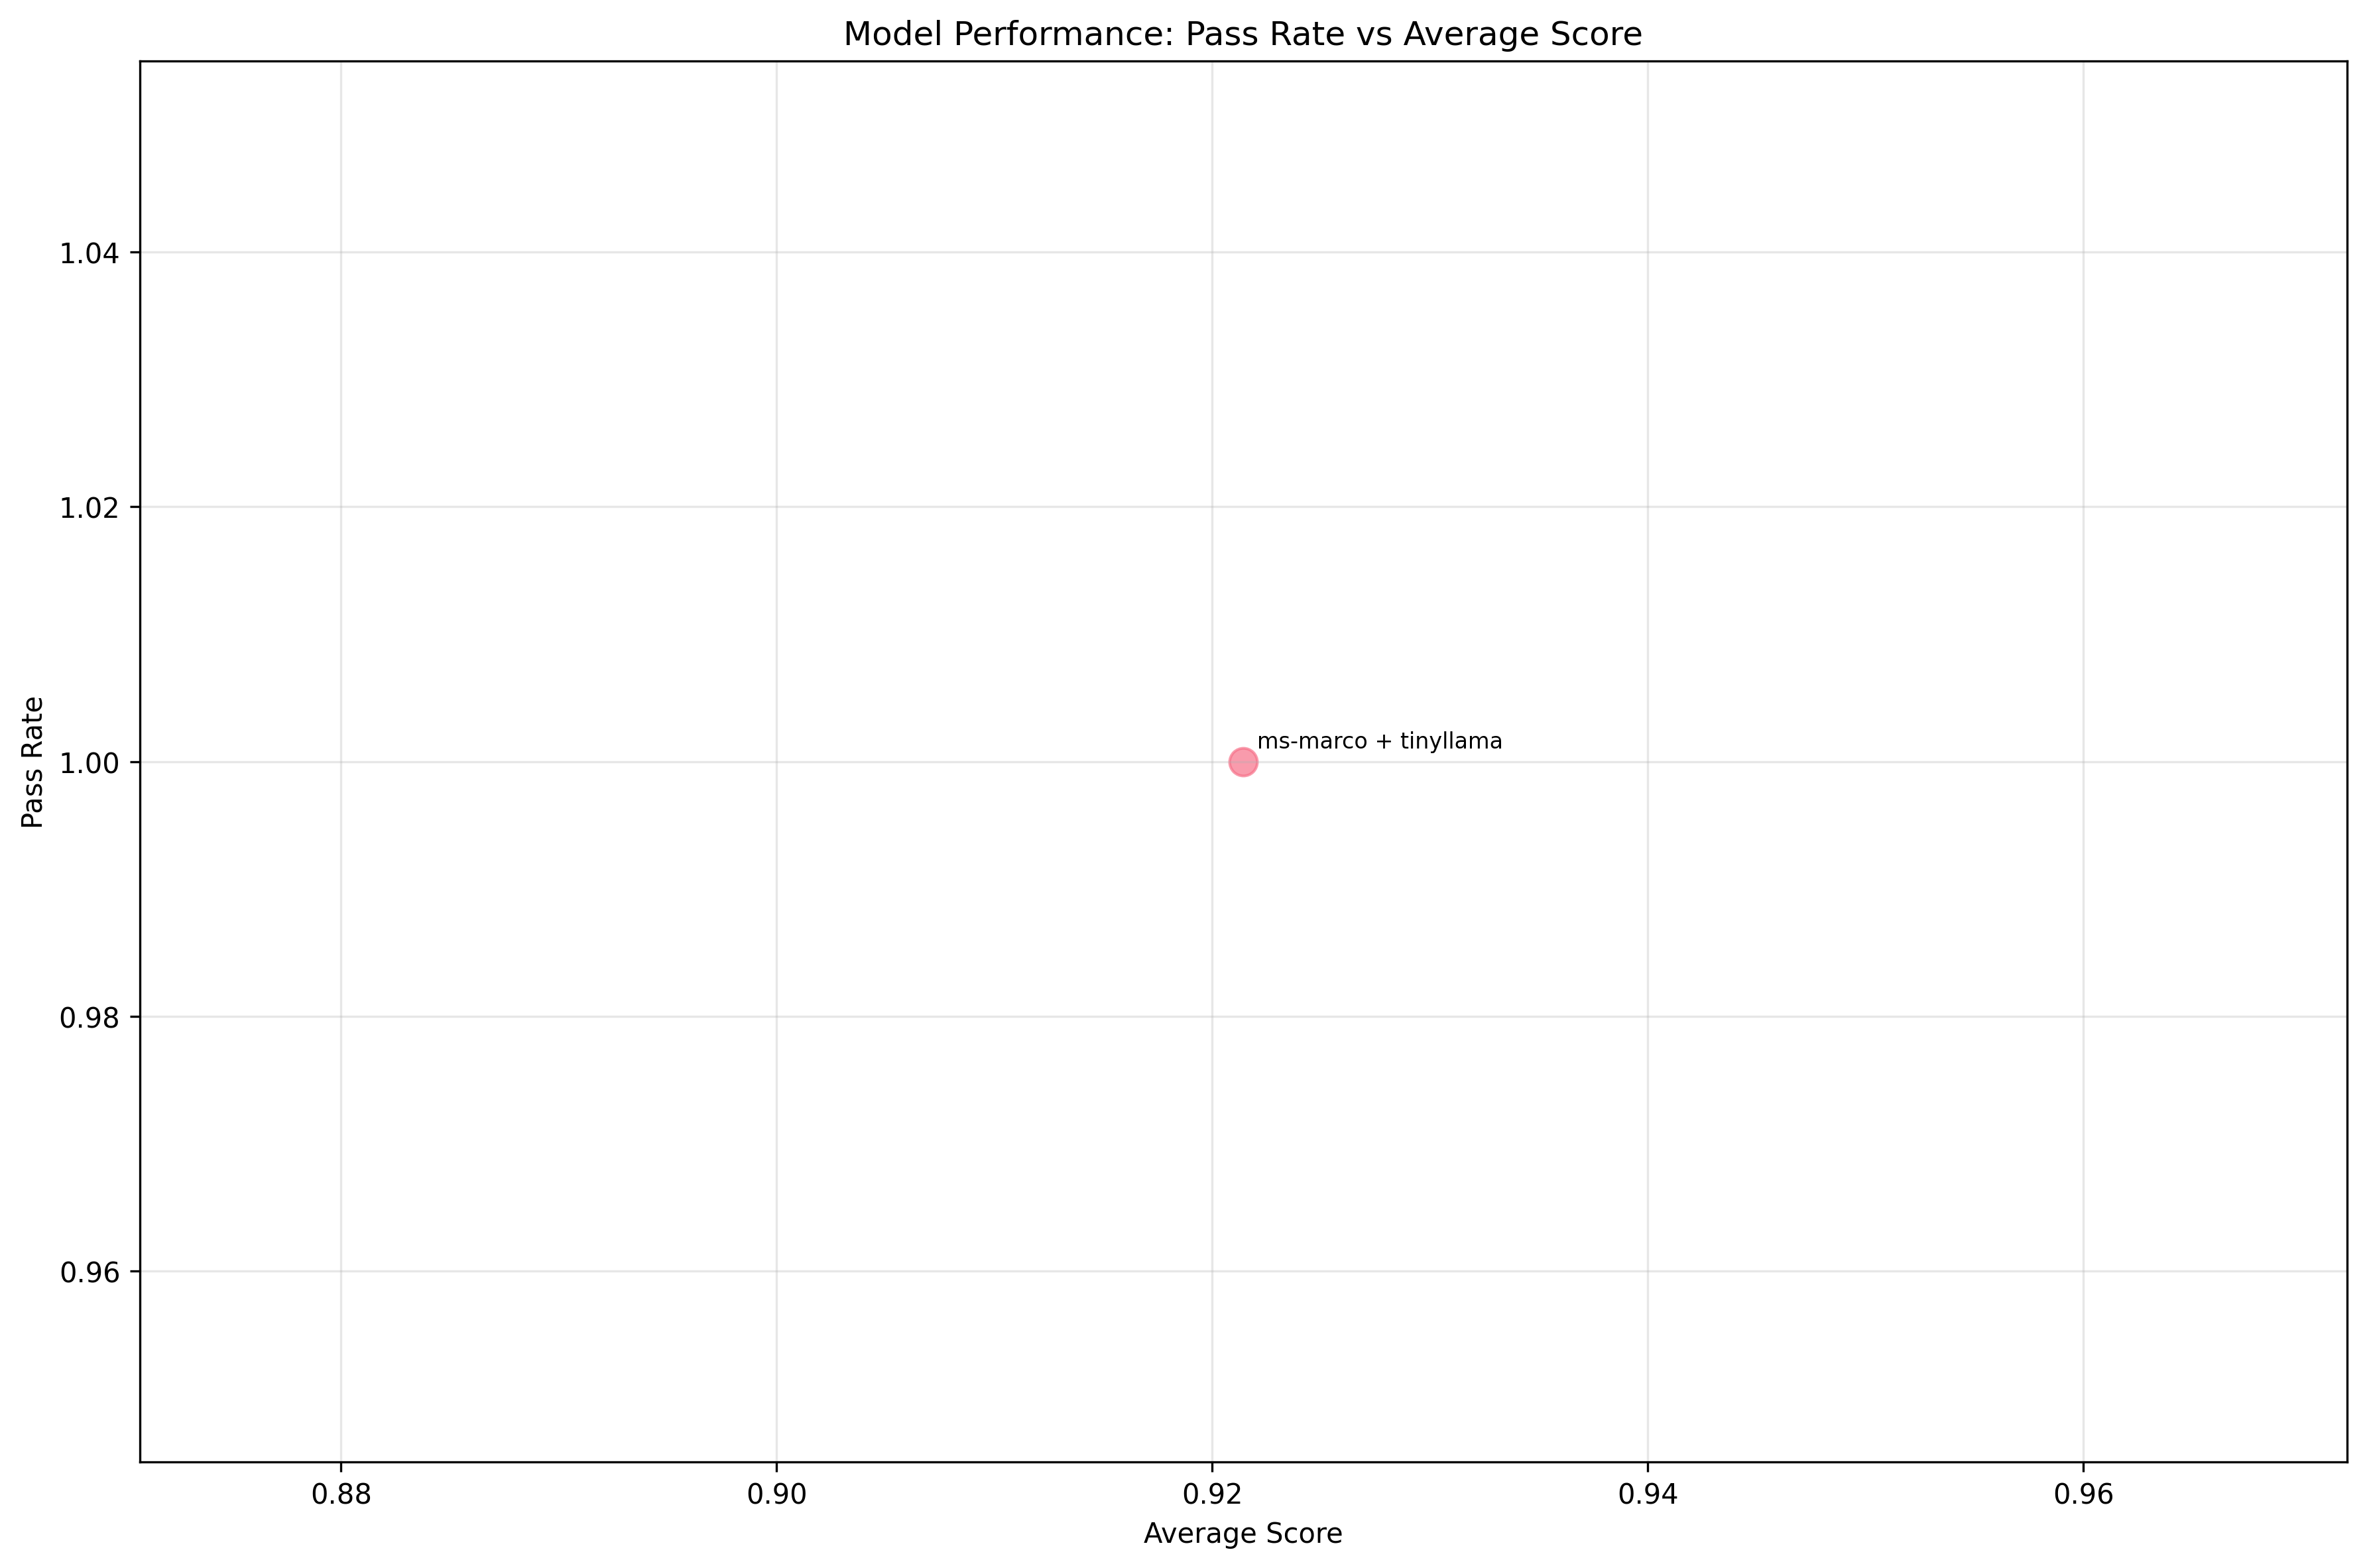
\includegraphics[width=\textwidth]{chap4_results/images/pass_rate_vs_score.png}
  \caption{Pass rate vs. average score by LLM. Highlights pairs that both pass reliably and score highly.}
  \label{fig:pass_rate_vs_score}
\end{figure}
    \chapter{Conclusions}
\textbf{This section should have a summary of the whole project.  The original aims and objective and whether these have been met should be discussed. It should include a section with a critique and a list of limitations of your proposed solutions.  Future work should be described, and this should not be marginal or silly (e.g.\ add machine learning models).  It is always good to end on a positive note (i.e.\ `Final Remarks').}

\section{Achieved Aims and Objectives}
\blindtext

\section{Critique and Limitations}
\blindtext

\section{Future Work}
\blindtext

\section{Final Remarks}
\blindtext

    % chap6_unused folder preserved for potential future content
    \appendix
        \chapter{Code Listings and Implementation Details}
\label{appendix:code}

This appendix contains key code snippets, implementation details, and technical documentation for the Clinical RAG Chatbot system.

\section{Core RAG Pipeline Implementation}

The following sections present the main components of the Clinical RAG system implementation:

\subsection{Document Processing and Chunking}
% Core text processing and chunking algorithms

\subsection{Vector Embeddings and Storage}
% Embedding generation and FAISS vector store implementation

\subsection{Retrieval and Context Management}
% Context retrieval and anti-hallucination measures

\section{API Implementation}

\subsection{Flask Backend Endpoints}
% Main API routes for chat functionality

\subsection{Error Handling and Logging}
% Comprehensive error management system

\section{Frontend Interface}

\subsection{React Chat Components}
% Material-UI chat interface implementation

\subsection{State Management}
% Frontend state handling for conversations

\section{Data Processing Scripts}

\subsection{MIMIC-IV Data Loading}
% Database connection and data extraction

\subsection{Text Preprocessing Pipeline}
% Clinical text preprocessing and normalization

\blindtext

        \chapter{Dataset Samples and Clinical Data}
\label{appendix:dataset}

This appendix presents sample data from the MIMIC-IV clinical database and demonstrates the structure and characteristics of the clinical text used in the RAG system.

\section{MIMIC-IV Database Overview}

The Medical Information Mart for Intensive Care IV (MIMIC-IV) database provides the clinical foundation for this research. This section describes the database structure and the specific tables utilized.

\subsection{Database Schema}
% Description of MIMIC-IV tables used:
% - admissions: Patient admission records
% - diagnoses\_icd: ICD diagnosis codes
% - procedures\_icd: Medical procedure codes
% - prescriptions: Medication prescriptions
% - labevents: Laboratory test results
% - microbiologyevents: Microbiology culture results

\section{Sample Clinical Records}

\subsection{Admission Records}
% Sample anonymized admission data showing patient demographics and admission details

\subsection{Diagnostic Information}
% Sample ICD diagnosis codes with descriptions and clinical context

\subsection{Procedure Documentation}
% Sample procedure records demonstrating clinical documentation patterns

\section{Text Preprocessing Examples}

\subsection{Raw Clinical Text}
% Examples of unprocessed clinical notes showing original formatting

\subsection{Processed and Chunked Documents}
% Examples showing text after preprocessing, cleaning, and semantic chunking

\section{Data Statistics}

\subsection{Dataset Characteristics}
Statistics about the clinical text corpus used in the RAG system:
% - Total documents: X
% - Average document length: Y tokens
% - Vocabulary size: Z unique terms
% - Clinical entity distribution
% - Document type breakdown

\blindtext

        \chapter{Evaluation Metrics and Results}
\label{appendix:evaluation}

This appendix provides detailed evaluation results, performance metrics, and statistical analysis of the Clinical RAG Chatbot system.

\section{Evaluation Framework}

\subsection{Metrics Definition}
Comprehensive evaluation metrics used to assess the RAG system:
% - Retrieval accuracy metrics (Precision@k, Recall, F1)
% - Response quality measures (BLEU, ROUGE, BERTScore)
% - Clinical relevance scoring
% - User satisfaction metrics

\subsection{Test Dataset}
% Description of evaluation dataset:
% - Gold standard questions from clinical experts
% - Expert-annotated responses
% - Clinical scenario coverage (diagnoses, treatments, procedures)

\section{Quantitative Results}

\subsection{Retrieval Performance}
% Statistical results for document retrieval:
% - Precision@1: X\%
% - Precision@5: Y\%
% - Recall@10: Z\%
% - Mean Reciprocal Rank (MRR): W

\subsection{Response Quality Metrics}
% Automated evaluation scores:
% - BLEU-4 score: A
% - ROUGE-L score: B
% - BERTScore F1: C
% - Clinical accuracy: D\%

\section{Qualitative Analysis}

\subsection{Expert Evaluation}
% Results from clinical expert reviews:
% - Medical accuracy assessment
% - Clinical relevance scoring (1-5 scale)
% - Safety evaluation results
% - Content appropriateness ratings

\subsection{User Study Results}
% User experience evaluation with healthcare professionals:
% - System Usability Scale (SUS) scores
% - Task completion success rates
% - Time-to-answer metrics
% - Error categorization and frequency

\section{Comparative Analysis}

\subsection{Baseline Comparisons}
% Performance comparison with baseline systems:
% - Traditional keyword search
% - Non-RAG conversational AI
% - Existing clinical QA systems
% - Human expert benchmarks

\subsection{Ablation Studies}
% Component-wise performance analysis:
% - Embedding model comparison (BioBERT vs. BioLORD vs. E5)
% - Chunk size optimization (128, 256, 512 tokens)
% - Anti-hallucination effectiveness
% - Context length impact on accuracy

\blindtext

        \chapter{User Interface Screenshots}
\label{appendix:ui}

This appendix contains screenshots and visual examples of the Clinical RAG Chatbot user interface, demonstrating the system's functionality and user experience.

% TODO: Add screenshots of:
% - Chat interface
% - Response formatting
% - Error handling
% - System prompts
% - Configuration screens

\blindtext % Remove this when adding actual content

        \chapter{Installation and Setup Guide}
\label{appendix:setup}

This appendix provides detailed instructions for installing, configuring, and running the Clinical RAG Chatbot system.

\section{System Requirements}

% TODO: Add system requirements
% - Python version
% - Hardware requirements
% - Software dependencies

\section{Installation Steps}

% TODO: Add step-by-step installation guide
% - Environment setup
% - Package installation
% - Database configuration
% - Model setup

\section{Configuration}

% TODO: Add configuration details
% - Environment variables
% - Configuration files
% - API keys setup

\section{Running the System}

% TODO: Add running instructions
% - Starting the backend
% - Starting the frontend
% - Accessing the application

\blindtext % Remove this when adding actual content


{\backmatter
    % Bibliography
    \if@openright\cleardoublepage\else\clearpage\fi
    \bibliographystyle{mmu-plainnat} %% MMU specific plainnat style
    {\footnotesize\bibliography{chap1_intro/introduction_biblio,chap2_lit_review/background_and_lit_overview_biblio,chap3_methodology/materials_and_methods_biblio,chap4_results/results_and_discussion_biblio,chap5_conclusions/conclusions_biblio}}
	\printindex
}

\end{document}

%%% The End %%%